\documentclass{standalone}
\usepackage{tikz}
\usepackage{ctex,siunitx,ninecolors}
\usepackage{tkz-euclide}
\usepackage{amsmath}
\usetikzlibrary{patterns, calc}
\usetikzlibrary {decorations.pathmorphing, decorations.pathreplacing, decorations.shapes,}
\begin{document}
\small
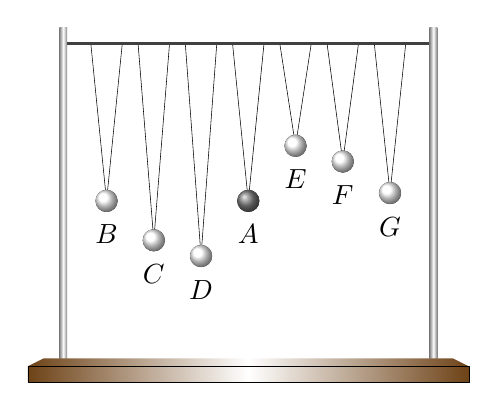
\begin{tikzpicture}[>=stealth,thick]
  \tkzDefPoints{.5/3/B1, .9/3/B2, 1.1/3/C1, 1.5/3/C2, 1.7/3/D1, 2.1/3/D2, 2.3/3/A1, 2.7/3/A2, 2.9/3/E1, 3.3/3/E2, 3.5/3/F1, 3.9/3/F2, 4.1/3/G1, 4.5/3/G2}
  \tkzDefPoints{.7/1/B, 1.3/.5/C, 1.9/.3/D, 2.5/1/A, 3.1/1.7/E, 3.7/1.5/F, 4.3/1.1/G}
  \tkzDrawSegments(B,B1 B,B2 A,A1 A,A2 C,C1 C,C2 D,D1 D,D2 E,E1 E,E2 F,F1 F,F2 G,G1 G,G2)
  \tkzLabelPoints[below=5pt](A,B,C,D,E,F,G)
  \foreach \x in {B,C,D,E,F,G}
  {
    \fill[ball color=white](\x) circle(4pt);
  }
  \fill[ball color=gray](A) circle(4pt);
  \draw[darkgray](0+.2,3)--(5-.2,3);
  \fill[right color=gray,left color=gray,middle color=white](0.1,3.2) rectangle (.2,-1);
  \fill[right color=gray,left color=gray,middle color=white](5-.1,3.2) rectangle (5-.2,-1);
  \tkzDefPoints{-.1/-1/a, 5.1/-1/b, -.3/-1.1/c, 5.3/-1.1/d, -.3/-1.3/c', 5.3/-1.3/d'}
  \tkzDrawPolygon[draw=none,right color=brown3,left color=brown3,middle color=white](a,b,d,c)
  \tkzDrawPolygon[ultra thin,right color=brown3,left color=brown3,middle color=white](d,c,c',d')
\end{tikzpicture}
\end{document}